\subsection{OPC-UA}
\label{subsection:opc-ua}
    The open platform communications unified architecture (OPC-UA) is published by the OPC Foundation, which with over 900 members is one of the world's leading organizations for interoperability solutions based on OPC specifications. It is an open information exchange standard for secure, reliable, manufacturer- and platform-independent industrial communications and has not only been the connectivity standard for nearly three decades but is still the most widely used open standard in the manufacturing industry. 

    The first OPC standard was named \textbf{O}LE \textbf{P}rocess \textbf{C}ontrol with ``OLE'' standing for Object Linking and Embedding. It enabled PLC controllers to deliver live data, alarms and historical data already back in 1996. In 2003 the OPC foundation started separating services from data and created OPC-UA as a service-oriented architecture which was later officially released in 2008 after verification with the goal to deliver a secure and reliable information exchange from sensors through to IT enterprise systems. In 2012 the standard was accepted as an International Electrotechnical Commission (IEC) standard called IEC62541.

    OPC-UA aims to address typical needs in smart manufacturing or Industry 4.0 like the need for standardized data connectivity and interoperability while being independent of both the device manufacturers and the operating systems used on the devices. Also, both horizontal (same layer, e.g. machine to machine on a shop floor) and vertical (across layers, e.g. device to cloud) data communications are supported by OPC-UA. Other interesting features of OPC-UA include the ability to scale from small microcontrollers with a footprint of around 15 kB up to multicore hardware. OPC-UA also provides mechanisms for application and user authentication, both for software and hardware systems. With object modeling, data can be described in a semantic way. Resources, also referred to as nodes, in the system are represented as objects with variables, methods, events and relationships to other objects. OPC-UA also supports automatic service and machine discovery while keeping independence of the transport method. Note that these are just some of the many requirements OPC-UA aims to satisfy. While this obviously results in a very rich and featureful standard, it also introduces lots of complexity and overhead that might be overkill in many scenarios. The OPC-UA is hence composed of 24 parts and the specification over 1200 pages long \cite{opc_foundation_interop}. When numerous and heterogeneous applications and devices from a variety of vendors are connected, OPC-UA becomes more and more challenging due to the high complexity and sheer length of the specification \cite{hivemq_opcua_vs_mqtt_sparkplug}.

    \begin{figure}[htbp]
        \centering
        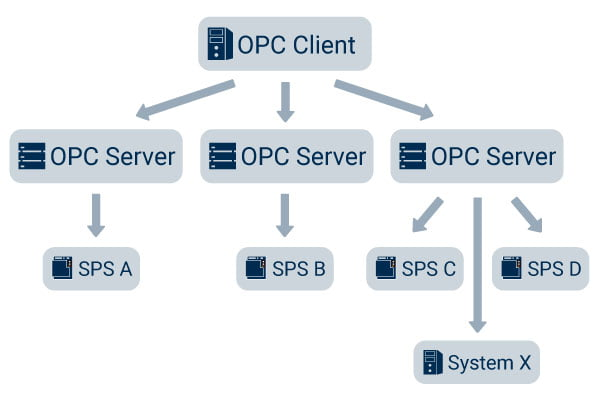
\includegraphics[width=0.6\textwidth]{img/opc-ua-cs-img.jpeg}
        \caption{OPC-UA Client Server Architecture \cite{rinke_was_2022}}
        \label{figure:opc-ua-cs-arch}
    \end{figure}

    \noindent OPC-UA has discovered and dealt with the shortcomings like point-to-point integrations of the automation pyramid covered in \autoref{subsection:automation-pyramid}. The classic OPC-UA system is designed upon a client/server architecture as shown in \autoref{figure:opc-ua-cs-arch} and uses TCP/IP and HTTP/SOAP. OPC-UA servers are responsible for converting the hardware communication protocols so that device data can be accessed by OPC-UA clients in a standardized way. Clients can decide when and which data the servers should retrieve from underlying systems like PLCs by polling on a configured interval. This is very simple since all resources (nodes) are individually addressable and (optionally) structured as data objects since OPC-UA supports object modeling. Nodes in the system are also automatically discovered. 
    
    This client/server model has its downsides though, one of them being, that the issue of point-to-point integrations is still a thing. While OPC-UA provides a standard format for communication, OPC-UA clients still communicate through direct bidirectional connections which results in similar problems as described for the automation pyramid in \autoref{subsection:automation-pyramid}. Apart from the point-to-point integrations, the biggest issue is scalability, which can be traced back to the architectural decision for a client-server model. Each OPC-UA client creates $n$ direct subscriptions/sessions to $m$ OPC-UA servers. The clients periodically request updates which is often referred to as ``polling''. As the number of clients and subscriptions increases the servers will experience higher processing loads while the network traffic becomes more demanding. This can quickly lead to scalability issues \cite{hivemq_opcua_vs_mqtt_sparkplug, manditereza_key_nodate}. 

    For these reasons, today's most widely used variant of the OPC standards is ``OPC-UA PubSub over MQTT'' which was released in 2018. The protocol MQTT will be further discussed in \autoref{subsubsection:mqtt}. With this variant, a separation between publishers and subscribers is implemented. The system is also re-engineered from a client/server architecture to an event-driven architecture, which addresses the scalability challenges. For today's IIoT systems, the PubSub variant of OPC-UA should always be preferred over the client/server model. It enables OPC-UA systems to scale from the edge up to the cloud. An MQTT broker acts as the single source of truth and enables all components in the system to access all data. This system architecture and its benefits will be discussed further in \autoref{section:unified-namespace}. The modern OPC-UA PubSub over MQTT standard also provides reference architectures for the large cloud providers like ``Microsoft Azure'', ``Amazon Web Services'' or ``Google Cloud Platform''. Through this new standard, most issues of the automation pyramid (\autoref{subsection:automation-pyramid}) like data silos, point-to-point integrations and stifling of innovation are solved \cite{manditereza_key_nodate}.\newline

    In summary, OPC-UA is an open standard that aims to fulfill as many requirements of industrial IoT as possible. Because of standards in communication, object modeling, flexibility in protocols and acceptance in the industry, OPC-UA is still the most widely used open standard in IIoT systems in manufacturing. While the client/server model of OPC-UA shines in simplicity, the OPC-UA PubSub with MQTT model should be preferred for today's systems, since the client/server model is not fit for today's scale of such complex projects. Overall, while OPC-UA is capable of fulfilling almost any use case one might have regarding an IIoT system, it is a very large and complex standard and its complexity must be taken into account when thinking about applying OPC-UA in a project.  